% =============================================================================
% CÁC PHẦN NÂNG CAO KHÁC
% =============================================================================

\section{Các phần nâng cao khác}
\label{sec:nang-cao}

Phần này tóm tắt các tình huống kỹ thuật chính và giải pháp đã triển khai trong đồ án Crypto Analytics Platform.

\subsection{1. Xử lý Dữ liệu Thị trường Thời gian thực}

Trong hệ thống phân tích tài chính, dữ liệu giá là trái tim của nền tảng. Yêu cầu: xử lý dữ liệu real-time với độ trễ thấp, theo dõi đồng thời nhiều cặp tiền (BTC, ETH, SOL), và đảm bảo tính ổn định khi kết nối bị gián đoạn.

\textbf{Vấn đề với HTTP Polling}: (1) Lãng phí tài nguyên---phần lớn request trả về dữ liệu không đổi; (2) Độ trễ cao---luôn có độ trễ ít nhất bằng nửa chu kỳ poll; (3) Rate limit---sàn giới hạn số request (ví dụ 1200 req/phút), polling nhiều cặp tiền dễ bị chặn IP.

\textbf{Giải pháp---Market Service với WebSocket \& Event-Driven}:
\begin{itemize}
    \item \textbf{WebSocket Ingestion}: Duy trì persistent connection với Binance Stream, đăng ký stream (vd. \texttt{btcusdt@kline\_1m}), nhận push-based thay vì poll.
    \item \textbf{Hub Pattern}: Pub/Sub nội bộ fan-out dữ liệu đến nhiều đích---Frontend WebSocket, Kafka topic \texttt{market\_price\_updates}, PostgreSQL.
    \item \textbf{Tự phục hồi}: Auto-reconnect với exponential backoff (1s, 2s, 4s...); graceful degradation---nếu Kafka lỗi tạm thời, luồng WebSocket cho client vẫn hoạt động.
\end{itemize}

Luồng điển hình: Giá thay đổi $\to$ Market Service nhận event vài ms $\to$ Parse và chuẩn hóa $\to$ Phân phối song song (WebSocket clients, Kafka, DB).

\begin{figure}[H]
\centering
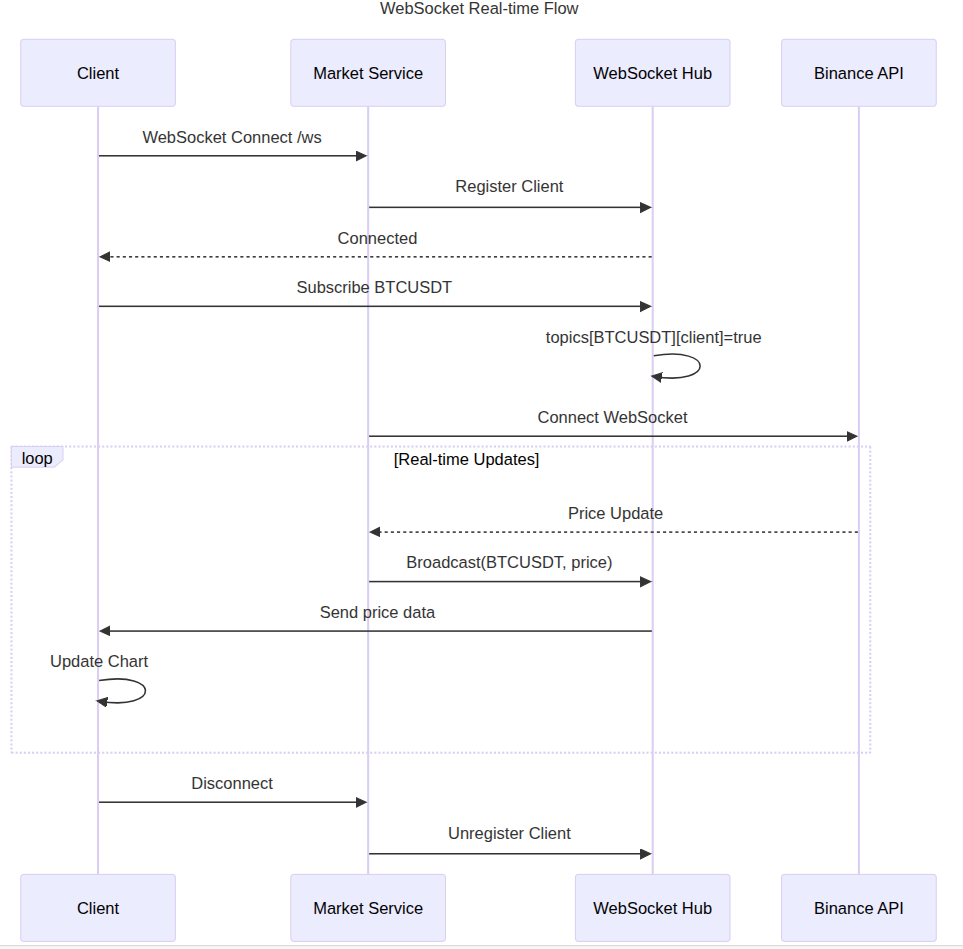
\includegraphics[width=0.9\textwidth]{sequence/sequence_websocket_flow.png}
\caption{Luồng WebSocket: Binance $\to$ Market Service $\to$ Clients}
\end{figure}

\subsection{2. Thu thập Tin tức với AI-Powered Crawler}

Cần thu thập tin tức tài chính từ hàng trăm website; nhiều trang dùng SPA (JavaScript render), cấu trúc HTML thường xuyên thay đổi. Crawler truyền thống (XPath/CSS cố định) dễ vỡ khi một class name thay đổi, chi phí bảo trì cao.

\textbf{Giải pháp---Crawler Service (Golang)}:
\begin{itemize}
    \item \textbf{RSS \& Multi-source}: Thu thập từ CoinDesk, CoinTelegraph, VNExpress, VnEconomy; goroutines crawl đồng thời.
    \item \textbf{Gemini AI CSS Selector}: Khi thêm nguồn mới, gửi HTML sample đến AI Service; Gemini (\texttt{gemini-1.5-flash}) phân tích cấu trúc và đề xuất selectors cho title, content, author, date; lưu vào DB (bảng \texttt{sources}); nếu selector fail (accuracy < 70\%), trigger re-analysis.
    \item \textbf{Kafka Event-Driven}: Bài viết mới được produce vào \texttt{news\_new\_article}; AI Service consume và phân tích sentiment; HTML cần phân tích selector vào \texttt{news\_analyze\_css\_selector}.
\end{itemize}

\textbf{Sentiment đa ngôn ngữ}: FinBERT (văn bản tài chính tiếng Anh) + PhoBERT (tiếng Việt). Pipeline: detect language $\to$ chọn model $\to$ tokenize và inference $\to$ extract attention weights cho keyword extraction. Top keywords từ attention scores cao nhất hỗ trợ người dùng hiểu nội dung chính.

\begin{figure}[H]
\centering
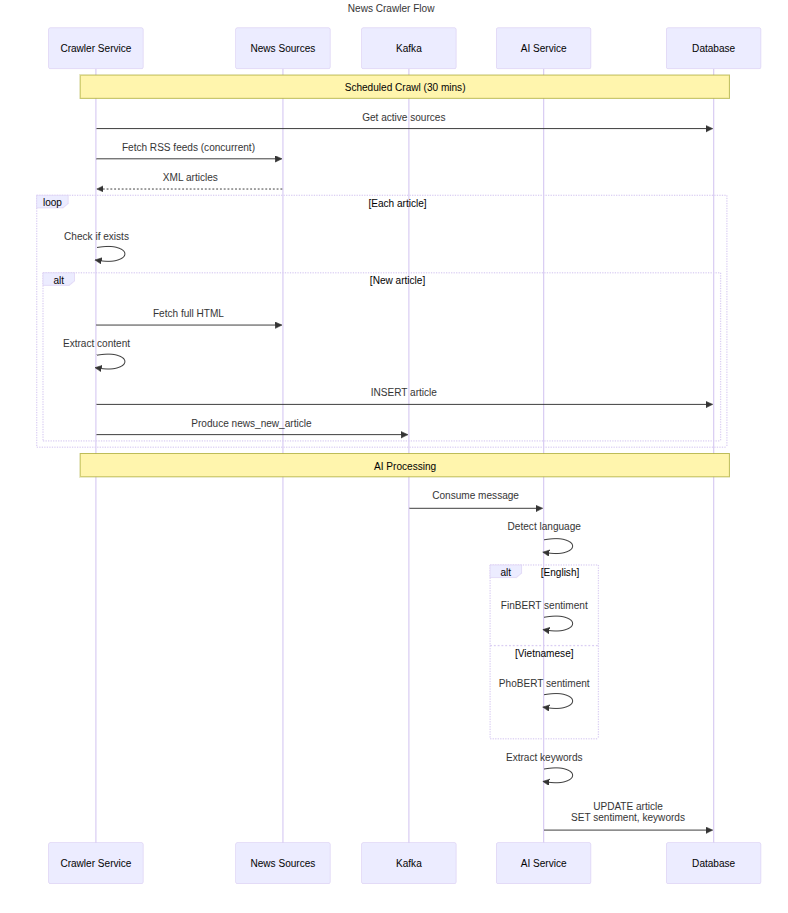
\includegraphics[width=0.9\textwidth]{sequence/sequence_crawler_flow.png}
\caption{Luồng Crawler với Kafka Event-Driven}
\end{figure}

\subsection{3. Bảo mật và Phân quyền}

Phát hiện truy cập bất thường---bypass API Gateway, JWT cũ vẫn hợp lệ, token replay. Hạn chế JWT alone: (1) Không thu hồi được sau khi cấp; (2) Thiếu Single Source of Truth; (3) Key rotation phức tạp.

\textbf{Giải pháp---Auth Service}:
\begin{itemize}
    \item \textbf{Access Token (JWT, short-lived)}: Claims \texttt{sub}, \texttt{email}, \texttt{role}, \texttt{iat}, \texttt{exp}; thời hạn 15--30 phút.
    \item \textbf{Refresh Token (opaque, lưu DB)}: Thời hạn dài hơn; lưu trong \texttt{refresh\_tokens}; mỗi lần \texttt{/auth/refresh} thành công thì rotate---vô hiệu hóa token cũ, cấp token mới.
    \item \textbf{Logout/Revoke}: Xóa refresh token trong DB; có thể blacklist JWT compromise.
    \item \textbf{Bcrypt} cho password hashing; token qua cookie \texttt{HttpOnly}, \texttt{Secure}, \texttt{SameSite}.
\end{itemize}

\textbf{Phân quyền VIP/Normal}: Middleware \texttt{RequireVIP} kiểm tra role từ JWT; tài khoản thường---xem biểu đồ, tin tức cơ bản; VIP/ADMIN---xem AI Prediction, SHAP explanation, sentiment scores, top keywords. \textbf{Zero-Trust}: API Gateway single entry point; validate mọi input; mTLS giữa services (khi triển khai Service Mesh).

\begin{figure}[H]
\centering
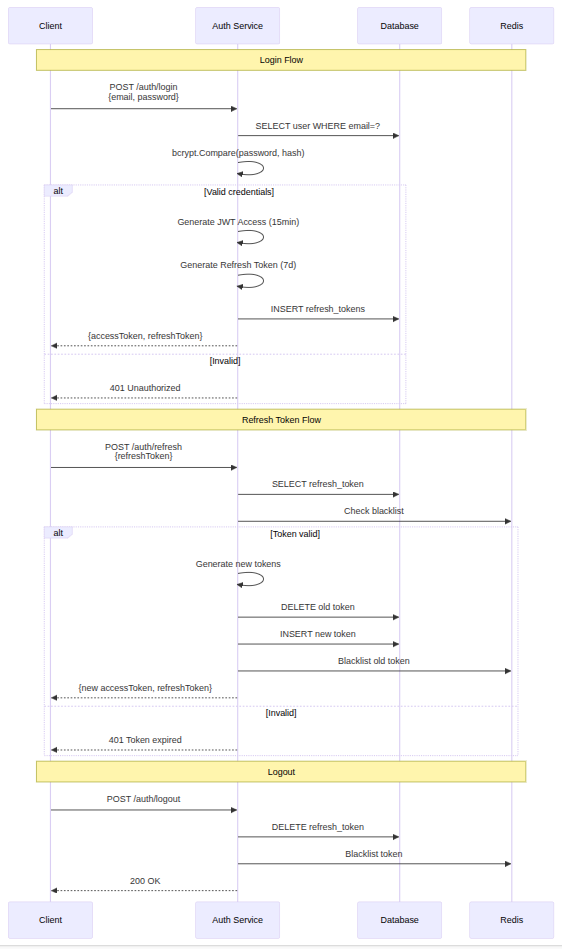
\includegraphics[width=0.85\textwidth]{sequence/sequence_auth_flow.png}
\caption{Luồng Authentication: JWT + Refresh Token}
\end{figure}

\subsection{4. Dự đoán Giá với Explainable AI (XAI)}

Yêu cầu: dự đoán xu hướng giá UP/DOWN (1h, 4h, 24h), kết hợp tin tức với giá lịch sử, và \textbf{giải thích} tại sao model đưa ra dự đoán. Black-box AI gây thiếu tin cậy, khó debug, không đạt chuẩn regulatory.

\textbf{Pipeline---XGBoost + SHAP}:
\begin{itemize}
    \item \textbf{Technical Features}: RSI, MACD, SMA, returns (\texttt{return\_1h}, \texttt{return\_24h}), volatility, lag features (\texttt{close\_lag\_1}, \texttt{close\_lag\_24}).
    \item \textbf{News Features}: Time-align tin tức với price theo hourly buckets; \texttt{sentiment\_mean}, \texttt{news\_count}, \texttt{sentiment\_ma\_24h}, \texttt{sentiment\_lag\_1h/6h}; merge left join, fill missing = 0.
    \item \textbf{Model}: XGBoost Regressor (200 trees, max\_depth=6, learning\_rate=0.05); train/test split 80/20 chronologically; target = future price sau \texttt{horizon\_hours}.
    \item \textbf{SHAP TreeExplainer}: Tính contribution từng feature; sort theo |SHAP|; top 10 features + phân loại news vs technical; \texttt{news\_influence\_pct} để người dùng thấy mức độ ảnh hưởng của tin tức.
\end{itemize}

\textbf{Top News \& Confidence}: Top 3 bài viết trong lookback window; keywords từ attention weights. Confidence = trung bình có trọng số của feature coverage, news availability, balance score (tỷ lệ news features gần 30\%).

\begin{figure}[H]
\centering
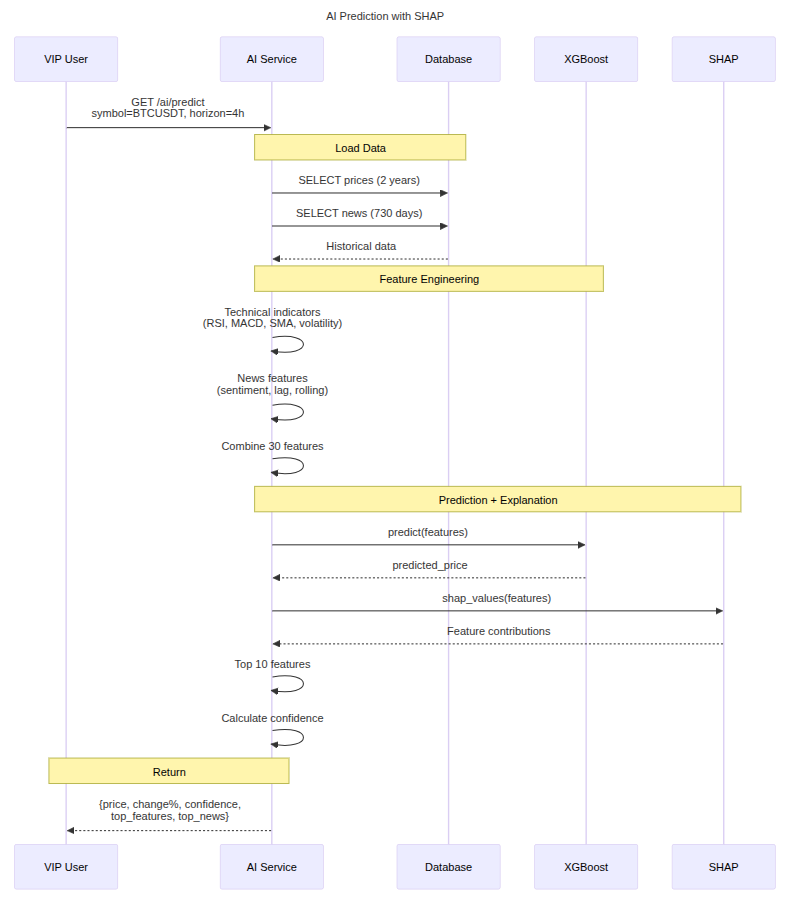
\includegraphics[width=0.9\textwidth]{sequence/sequence_ai_prediction_flow.png}
\caption{Luồng AI Prediction với SHAP XAI}
\end{figure}

\subsection{5. Topic-based WebSocket Hub}

Khi nhiều người dùng đồng thời kết nối WebSocket, cần cơ chế broadcast hiệu quả. Hub dùng \textbf{topic-based subscription}: mỗi client subscribe các topics (vd. \texttt{btcusdt@kline\_1m}, \texttt{ethusdt@kline\_5m}); server chỉ broadcast đến clients đã subscribe topic tương ứng, tránh gửi dữ liệu không liên quan.

\textbf{Mở rộng đa server}: (1) \textbf{Kafka}---mỗi Market instance publish vào topic; consumer redistribute đến WebSocket clients; (2) \textbf{Redis Pub/Sub}---các Hub instances subscribe channel; instance nhận dữ liệu publish lên Redis; instances khác nhận và broadcast local; (3) \textbf{Sticky Session}---Load balancer giữ client với cùng Market instance cho một symbol. Hệ thống hiện có Kafka producer \texttt{market\_price\_update} sẵn sàng cho mở rộng.

\begin{figure}[H]
\centering

\includegraphics[width=0.85\textwidth]{pattern_observer}
\caption{Topic-based WebSocket Hub}
\label{fig:nangcao-websocket}
\end{figure}

\subsection{6. Gemini AI CSS Selector \& Multi-language Sentiment}

\textbf{Gemini AI}: Workflow---Crawler gửi HTML sample qua Kafka topic \texttt{news\_analyze\_css\_selector}; AI Service gọi \texttt{gemini-1.5-flash} với prompt mô tả cấu trúc trang; model đề xuất CSS selectors cho title, link, content, author; validate và lưu vào bảng \texttt{sources}; lần crawl sau dùng selectors đã học. Khi website đổi layout, admin gọi \textit{Analyze} lại mà không cần sửa code.

\textbf{FinBERT + PhoBERT}: Tin tức có cả tiếng Anh và tiếng Việt. FinBERT (\texttt{yiyanghkust/finbert-tone}) chuyên văn bản tài chính en; PhoBERT (\texttt{wonrax/phobert-base-vietnamese-sentiment}) cho vi. Pipeline: langdetect $\to$ chọn model $\to$ tokenize (underthesea cho vi) $\to$ inference. Strategy pattern cho phép dễ thêm model mới.

\begin{figure}[H]
\centering

\includegraphics[width=0.75\textwidth]{pattern_strategy}
\caption{Strategy: FinBERT / PhoBERT}
\label{fig:nangcao-sentiment}
\end{figure}

\subsection{7. Event-driven với Kafka}

Các service giao tiếp qua Kafka topics: \texttt{news\_new\_article} (Crawler $\to$ AI), \texttt{news\_analyze\_css\_selector} (Crawler $\to$ AI cho HTML analysis), \texttt{market\_price\_update} (Market $\to$ AI/consumers). Lợi ích: \textbf{loose coupling}---Crawler và AI chạy bất đồng bộ; AI chậm không block Crawler; \textbf{scalability}---dễ thêm consumer mới (vd. notification service) mà không sửa Crawler; \textbf{reliability}---Kafka đảm bảo message delivery, có thể replay khi consumer fail.

\subsection{Tổng kết giải pháp}

\begin{table}[H]
\centering
\caption{Tóm tắt giải pháp kỹ thuật}
\begin{tabular}{|l|l|l|}
\hline
\textbf{Tình huống} & \textbf{Vấn đề} & \textbf{Giải pháp} \\
\hline
WebSocket Scale & Polling tốn tài nguyên & Hub + Topic-based + Kafka \\
\hline
Crawler & HTML thay đổi & Gemini AI selector, RSS \\
\hline
Security & JWT không revoke được & Refresh Token + DB \\
\hline
AI Prediction & Black-box & XGBoost + SHAP XAI \\
\hline
Multi-language & en/vi & FinBERT + PhoBERT \\
\hline
\end{tabular}
\end{table}
